\documentclass[11pt]{article}
\usepackage{mathblatt}
% gesetzt von werkzeuge/setzer.py (Sorte selbst) aus dem Lernweg HMF
% und den Bankzeilen; Muster bau/proben/2026-10-09/hypotenuse-muster.
\usepackage{enumitem}
\usepackage{adjustbox,varwidth}
\newgeometry{a4paper,margin=18mm,top=15mm,bottom=20mm,footskip=9mm}
\pagestyle{fancy}\fancyhf{}\renewcommand{\headrulewidth}{0pt}
\fancyfoot[L]{\footnotesize\color{mbgrau}HMF \textperiodcentered{} Vergleichen, Ordnen, Runden}
\fancyfoot[R]{\footnotesize\color{mbgrau}\thepage}
\setlength{\parskip}{3pt}
\renewcommand{\kreuz}[1]{\mbox{$\square$\ #1}\quad}
\newcommand{\kreuzl}[1]{\par\hangindent1.4em\hangafter1\noindent$\square$\ #1}
\newcommand{\aufg}[3]{\par\noindent\makebox[0pt][r]{#3}\begin{minipage}[t]{\linewidth}#1\end{minipage}\par}
\newcommand{\aufgg}[4]{\par\noindent\makebox[0pt][r]{#4}\begin{minipage}[t]{0.6\linewidth}\vspace{0pt}#1\end{minipage}\hfill
  \begin{minipage}[t]{0.37\linewidth}\vspace{0pt}\centering #2\end{minipage}\par}
\newcommand{\nr}[1]{\makebox[7mm][l]{\textbf{#1}}}
\newcommand{\lsg}[3]{\par\noindent\begin{minipage}[t]{9mm}\textbf{#1}\end{minipage}%
  \begin{minipage}[t]{52mm}\raggedright\bfseries\boldmath #2\end{minipage}\hspace{3mm}%
  \begin{minipage}[t]{\dimexpr\linewidth-64mm\relax}\raggedright\small #3\end{minipage}\par\vspace{4pt}}
\newlength{\kr}
\makeatletter
\newcommand{\karomerk}[2]{\protected@write\@auxout{}{\string\karoseite{#1}{#2}{\thepage}}}
\newcommand{\karoseite}[3]{\expandafter\xdef\csname karo@#1@#2\endcsname{#3}}
\newcommand{\karohinweis}[3]{\karomerk{h}{#1}\ifcsname karo@k@#1\endcsname
  \ifnum\csname karo@k@#1\endcsname=0\csname karo@h@#1\endcsname\relax#2\else#3\fi
  \else#3\fi}
\makeatother
\begin{document}

\noindent{\LARGE\bfseries Vergleichen, Ordnen, Runden}\par\smallskip
\noindent{\small\color{mbgrau}Selbstlernheft Klasse 6 \textperiodcentered{} mit Lösungsheft \textperiodcentered{} Kennung HMF}\par\medskip
\noindent\textbf{So nutzt du das Heft:} Lies im Abschnitt das Beispiel. Rechne dann die Aufgaben der Reihe nach und vergleiche jede sofort mit dem Lösungsheft. Kreuze „kann ich“ an, wenn du die letzte Aufgabe (\emph{Ziel}) allein schaffst.\par
\noindent Mehr Aufgaben zu einem Abschnitt: Kennung deinem Nachhilfelehrer schicken (z.\,B. „HMF mehr B“).\par\medskip
{\arrayrulecolor{mbgrau}\renewcommand{\arraystretch}{1.3}
\noindent\begin{tabular}{|>{\bfseries}p{10mm}|p{112mm}|>{\raggedleft\arraybackslash}p{10mm}|>{\centering\arraybackslash}p{14mm}|}\hline
\rowcolor{black!8} & \textbf{Abschnitt} & \textbf{Seite} & \textbf{kann ich}\\\hline
A & Vergleichen und ordnen & \pageref{s:A} & $\square$\\\hline
B & Runden & \pageref{s:B} & $\square$\\\hline
C & Dazwischen und genau in der Mitte & \pageref{s:C} & $\square$\\\hline
D & Bruch, Prozent, Quadrat: erst umwandeln & \pageref{s:D} & $\square$\\\hline
T & Probetest & \pageref{s:T} & $\square$\\\hline
\end{tabular}}\par\bigskip

\begin{tcolorbox}[colback=mbkasten,colframe=mbgrau,boxrule=0.5pt,arc=1mm,left=3mm,right=3mm,top=2mm,bottom=2mm,title={\bfseries Formel auf einen Blick},coltitle=black,colbacktitle=black!10]
{\Large $0{,}1 = \dfrac{1}{10}$ \qquad $0{,}01 = \dfrac{1}{100}$ \qquad $0{,}001 = \dfrac{1}{1000}$}\par\medskip
In Worten: Jede Stelle nach rechts ist zehnmal kleiner als die davor.\par\medskip
\end{tcolorbox}
\medskip\noindent\textbf{Typische Fehler – so nicht}\par\smallskip
\noindent\nr{$\times$}Nach der Länge verglichen: $2{,}09$ ist nicht größer als $2{,}1$, auch wenn $9 > 1$ ist.\par
\noindent\nr{$\times$}Quadrat verdoppelt: $0{,}4^2$ ist nicht $0{,}8$, sondern $0{,}4 \cdot 0{,}4 = 0{,}16$.\par
\clearpage\label{s:A}\noindent\colorbox{black!12}{\makebox[10mm]{\Large\bfseries\strut A}}\hspace{3mm}{\Large\bfseries Vergleichen und ordnen}\par\smallskip
\noindent Hänge Nullen an, bis beide Zahlen gleich viele Stellen nach dem Komma haben – das ändert den Wert nicht. Dann vergleichst du Stelle für Stelle von links: Die erste Stelle, an der sie sich unterscheiden, entscheidet.\par\medskip
\noindent\textbf{Formel}\par\nopagebreak\noindent\hspace*{4mm}\begin{minipage}{\dimexpr\linewidth-4mm\relax}$3{,}7 = 3{,}70 = 3{,}700$ \par\vspace{4pt} $3{,}70 > 3{,}68$, \ denn 7 Zehntel $>$ 6 Zehntel\end{minipage}\par\medskip
\noindent\textbf{Beispiel}\quad Ordne von klein nach groß: $0{,}5$; \ $0{,}45$; \ $0{,}405$; \ $0{,}54$.\par\smallskip
\noindent\par\noindent\hangindent6mm\hangafter1\makebox[6mm][l]{\textbf{1}}Hänge Nullen an, bis alle drei Stellen nach dem Komma haben: $0{,}500$; \ $0{,}450$; \ $0{,}405$; \ $0{,}540$.\par\smallskip\par\noindent\hangindent6mm\hangafter1\makebox[6mm][l]{\textbf{2}}Vergleiche von links. Einer: überall 0. Zehntel: 4 bei $0{,}450$ und $0{,}405$, 5 bei $0{,}500$ und $0{,}540$.\par\smallskip\par\noindent\hangindent6mm\hangafter1\makebox[6mm][l]{\textbf{3}}Gleiche Zehntel: Die Hundertstel entscheiden. $0{,}405 < 0{,}450$ \ und \ $0{,}500 < 0{,}540$.\par\smallskip\par\noindent\hangindent6mm\hangafter1\makebox[6mm][l]{\textbf{4}}Ohne die angehängten Nullen: $0{,}405 < 0{,}45 < 0{,}5 < 0{,}54$.\par\smallskip\par\medskip
\noindent\textbf{Aufgaben}\hspace{1em}{\small\color{mbgrau}\karohinweis{A}{Rechne unten im Karo.}{Rechne auf einem extra Blatt.} Vergleiche jede Aufgabe gleich mit dem Lösungsheft.}\par\smallskip
\aufg{\hangindent7mm\hangafter1\nr{1.}Setze $<$ oder $>$ ein.\par\vspace{3pt} a)~$0{,}58$ \leerfeld $0{,}54$ \qquad b)~$4{,}62$ \leerfeld $4{,}26$ \qquad c)~$15{,}2$ \leerfeld $16{,}2$ \qquad d)~$0{,}071$ \leerfeld $0{,}017$}{}{}
\medskip
\aufg{\hangindent7mm\hangafter1\nr{2.}Hänge Nullen an. Setze dann $<$, $=$ oder $>$ ein.\par\vspace{3pt} a)~$0{,}7$ \leerfeld $0{,}69$ \qquad b)~$3{,}45$ \leerfeld $3{,}5$ \qquad c)~$0{,}41$ \leerfeld $0{,}405$ \qquad d)~$5{,}1$ \leerfeld $5{,}10$}{}{}
\medskip
\aufg{\hangindent7mm\hangafter1\nr{3.}Ordne von klein nach groß: $4{,}3$; \ $4{,}03$; \ $4{,}33$; \ $4{,}303$.}{}{}
\medskip
\aufg{\hangindent7mm\hangafter1\nr{4.}Ordne diesmal von groß nach klein: $5{,}08$; \ $5{,}8$; \ $5{,}008$; \ $5{,}088$.}{}{}
\medskip
\aufg{\hangindent7mm\hangafter1\nr{5.}Fünf Kinder schwimmen $50$\,m. Die Zeiten: Ela $41{,}8$\,s, Finn $41{,}08$\,s, Gül $41{,}75$\,s, Hannes $42{,}1$\,s, Ida $41{,}1$\,s. Wer bekommt Silber (Platz 2), wer Bronze (Platz 3)?}{}{{\scriptsize\color{mbgrau}Ziel\hspace{2mm}}}
\medskip
\par\vspace{3mm}\setlength{\kr}{\dimexpr\pagegoal-\pagetotal-10mm\relax}%
\ifdim\kr>12mm\karomerk{k}{A}\noindent{\scriptsize\color{mbgrau}Platz zum Rechnen}\par\nointerlineskip\vspace{1mm}\noindent
\begin{tikzpicture}\clip (0,0) rectangle ({\linewidth-0.5mm},\kr);\draw[black!16,line width=0.3pt,step=5mm] (0,0) grid (\linewidth,\kr);\end{tikzpicture}\fi\par
\clearpage\label{s:B}\noindent\colorbox{black!12}{\makebox[10mm]{\Large\bfseries\strut B}}\hspace{3mm}{\Large\bfseries Runden}\par\smallskip
\noindent Beim Runden entscheidet die Ziffer rechts von der Rundungsstelle: Bei 0 bis 4 bleibt die Rundungsstelle, bei 5 bis 9 wird sie um 1 größer; alles dahinter fällt weg. Auf Cent oder Zentimeter heißt auf Hundertstel.\par\medskip
\noindent\textbf{Formel}\par\nopagebreak\noindent\hspace*{4mm}\begin{minipage}{\dimexpr\linewidth-4mm\relax}auf Zehntel: \ $7{,}24 \approx 7{,}2$ \qquad $7{,}25 \approx 7{,}3$ \par\vspace{4pt} 10 Zehntel $=$ 1 Einer, \ 10 Hundertstel $=$ 1 Zehntel\end{minipage}\par\medskip
\noindent\textbf{Beispiel}\quad Runde $5{,}763$ auf Zehntel und auf Hundertstel. Runde $6{,}97$ auf Zehntel.\par\smallskip
\noindent\par\noindent\hangindent6mm\hangafter1\makebox[6mm][l]{\textbf{1}}Auf Zehntel: Rechts vom Zehntel steht die 6. Bei 5 bis 9 aufrunden: $5{,}763 \approx 5{,}8$.\par\smallskip\par\noindent\hangindent6mm\hangafter1\makebox[6mm][l]{\textbf{2}}Auf Hundertstel: Rechts vom Hundertstel steht die 3. Bei 0 bis 4 abrunden: $5{,}763 \approx 5{,}76$.\par\smallskip\par\noindent\hangindent6mm\hangafter1\makebox[6mm][l]{\textbf{3}}$6{,}97$ auf Zehntel: Rechts steht die 7, also aufrunden: 9 Zehntel $+$ 1 Zehntel $=$ 10 Zehntel $=$ 1 Einer.\par\smallskip\par\noindent\hangindent6mm\hangafter1\makebox[6mm][l]{\textbf{4}}Der Einer wird 7, an der Zehntelstelle bleibt die 0 stehen: $6{,}97 \approx 7{,}0$.\par\smallskip\par\medskip
\noindent\textbf{Aufgaben}\hspace{1em}{\small\color{mbgrau}\karohinweis{B}{Rechne unten im Karo.}{Rechne auf einem extra Blatt.} Vergleiche jede Aufgabe gleich mit dem Lösungsheft.}\par\smallskip
\aufg{\hangindent7mm\hangafter1\nr{1.}Runde auf Zehntel.\par\vspace{3pt} a)~$2{,}73$ \qquad b)~$5{,}48$ \qquad c)~$0{,}35$ \qquad d)~$8{,}04$}{}{}
\medskip
\aufg{\hangindent7mm\hangafter1\nr{2.}Runde auf Hundertstel.\par\vspace{3pt} a)~$1{,}234$ \qquad b)~$6{,}078$ \qquad c)~$12{,}465$ \qquad d)~$0{,}555$}{}{}
\medskip
\aufg{\hangindent7mm\hangafter1\nr{3.}Runde. Achte darauf, was aus 10 Zehnteln oder 10 Hundertsteln wird.\par\vspace{3pt} a)~$2{,}97$ auf Zehntel \par b)~$9{,}96$ auf Zehntel \par c)~$3{,}998$ auf Hundertstel \par d)~$0{,}95$ auf Zehntel}{}{}
\medskip
\aufg{\hangindent7mm\hangafter1\nr{4.}Runde die Größen.\par\vspace{3pt} a)~$2{,}346$\,€ auf Cent \par b)~$3{,}96$\,kg auf Zehntel \par c)~$1{,}784$\,m auf Zentimeter \par d)~$12{,}05$\,s auf Zehntel}{}{}
\medskip
\aufg{\hangindent7mm\hangafter1\nr{5.}Mia kauft Käse. Die Waage rechnet einen Preis von $4{,}865$\,€ aus. Auf dem Bon steht der Preis auf Cent gerundet. Mia hat genau $4{,}85$\,€ dabei. Reicht ihr Geld?}{}{{\scriptsize\color{mbgrau}Ziel\hspace{2mm}}}
\medskip
\par\vspace{3mm}\setlength{\kr}{\dimexpr\pagegoal-\pagetotal-10mm\relax}%
\ifdim\kr>12mm\karomerk{k}{B}\noindent{\scriptsize\color{mbgrau}Platz zum Rechnen}\par\nointerlineskip\vspace{1mm}\noindent
\begin{tikzpicture}\clip (0,0) rectangle ({\linewidth-0.5mm},\kr);\draw[black!16,line width=0.3pt,step=5mm] (0,0) grid (\linewidth,\kr);\end{tikzpicture}\fi\par
\clearpage\label{s:C}\noindent\colorbox{black!12}{\makebox[10mm]{\Large\bfseries\strut C}}\hspace{3mm}{\Large\bfseries Dazwischen und genau in der Mitte}\par\smallskip
\noindent Zwischen zwei Dezimalzahlen liegen immer weitere: Hänge eine Null an, dann siehst du sie. Für die Mitte rechnest du ohne Komma und gehst den halben Abstand weiter.\par\medskip
\noindent\textbf{Formel}\par\nopagebreak\noindent\hspace*{4mm}\begin{minipage}{\dimexpr\linewidth-4mm\relax}Mitte $=$ kleinere Zahl $+$ Abstand $: 2$ \par\vspace{4pt} $1{,}3 = 1{,}30$ und $1{,}4 = 1{,}40$: \ dazwischen $1{,}31;\ 1{,}32;\ \ldots;\ 1{,}39$\end{minipage}\par\medskip
\noindent\textbf{Beispiel}\quad Welche Zahl liegt genau in der Mitte zwischen $2{,}3$ und $2{,}6$? Nenne noch eine Zahl, die dazwischen liegt.\par\smallskip
\noindent\begin{minipage}[t]{0.6\linewidth}\vspace{0pt}\par\noindent\hangindent6mm\hangafter1\makebox[6mm][l]{\textbf{1}}Hänge an beide Zahlen eine Null an: $2{,}30$ und $2{,}60$.\par\smallskip\par\noindent\hangindent6mm\hangafter1\makebox[6mm][l]{\textbf{2}}Lies sie ohne Komma (in Hundertsteln): $230$ und $260$.\par\smallskip\par\noindent\hangindent6mm\hangafter1\makebox[6mm][l]{\textbf{3}}Abstand: $260 - 230 = 30$. Die Hälfte: $15$. Mitte: $230 + 15 = 245$.\par\smallskip\par\noindent\hangindent6mm\hangafter1\makebox[6mm][l]{\textbf{4}}Komma zurück, so viele Stellen wie nach dem Anhängen: Mitte $= 2{,}45$.\par\smallskip\par\noindent\hangindent6mm\hangafter1\makebox[6mm][l]{\textbf{5}}Jede Zahl zwischen $230$ und $260$ liegt dazwischen, z.\,B. $231$, also $2{,}31$.\par\smallskip\end{minipage}\hfill
\begin{minipage}[t]{0.37\linewidth}\vspace{0pt}\centering 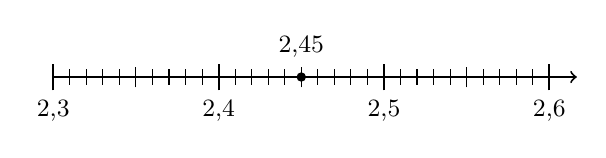
\begin{tikzpicture}[font=\small]\draw[->,line width=0.7pt] (0,0) -- (6.65,0);\draw[line width=0.7pt] (0.000,-0.17) -- (0.000,0.17);\node[below] at (0.000,-0.17) {$2{,}3$};\draw[line width=0.4pt] (0.210,-0.1) -- (0.210,0.1);\draw[line width=0.4pt] (0.420,-0.1) -- (0.420,0.1);\draw[line width=0.4pt] (0.630,-0.1) -- (0.630,0.1);\draw[line width=0.4pt] (0.840,-0.1) -- (0.840,0.1);\draw[line width=0.4pt] (1.050,-0.13) -- (1.050,0.13);\draw[line width=0.4pt] (1.260,-0.1) -- (1.260,0.1);\draw[line width=0.4pt] (1.470,-0.1) -- (1.470,0.1);\draw[line width=0.4pt] (1.680,-0.1) -- (1.680,0.1);\draw[line width=0.4pt] (1.890,-0.1) -- (1.890,0.1);\draw[line width=0.7pt] (2.100,-0.17) -- (2.100,0.17);\node[below] at (2.100,-0.17) {$2{,}4$};\draw[line width=0.4pt] (2.310,-0.1) -- (2.310,0.1);\draw[line width=0.4pt] (2.520,-0.1) -- (2.520,0.1);\draw[line width=0.4pt] (2.730,-0.1) -- (2.730,0.1);\draw[line width=0.4pt] (2.940,-0.1) -- (2.940,0.1);\draw[line width=0.4pt] (3.150,-0.13) -- (3.150,0.13);\draw[line width=0.4pt] (3.360,-0.1) -- (3.360,0.1);\draw[line width=0.4pt] (3.570,-0.1) -- (3.570,0.1);\draw[line width=0.4pt] (3.780,-0.1) -- (3.780,0.1);\draw[line width=0.4pt] (3.990,-0.1) -- (3.990,0.1);\draw[line width=0.7pt] (4.200,-0.17) -- (4.200,0.17);\node[below] at (4.200,-0.17) {$2{,}5$};\draw[line width=0.4pt] (4.410,-0.1) -- (4.410,0.1);\draw[line width=0.4pt] (4.620,-0.1) -- (4.620,0.1);\draw[line width=0.4pt] (4.830,-0.1) -- (4.830,0.1);\draw[line width=0.4pt] (5.040,-0.1) -- (5.040,0.1);\draw[line width=0.4pt] (5.250,-0.13) -- (5.250,0.13);\draw[line width=0.4pt] (5.460,-0.1) -- (5.460,0.1);\draw[line width=0.4pt] (5.670,-0.1) -- (5.670,0.1);\draw[line width=0.4pt] (5.880,-0.1) -- (5.880,0.1);\draw[line width=0.4pt] (6.090,-0.1) -- (6.090,0.1);\draw[line width=0.7pt] (6.300,-0.17) -- (6.300,0.17);\node[below] at (6.300,-0.17) {$2{,}6$};\fill (3.150,0) circle (1.7pt);\node[above] at (3.150,0.12) {$2{,}45$};\end{tikzpicture}\end{minipage}\par\medskip
\noindent\textbf{Aufgaben}\hspace{1em}{\small\color{mbgrau}\karohinweis{C}{Rechne unten im Karo.}{Rechne auf einem extra Blatt.} Vergleiche jede Aufgabe gleich mit dem Lösungsheft.}\par\smallskip
\aufg{\hangindent7mm\hangafter1\nr{1.}Gib eine Zahl an, die dazwischen liegt.\par\vspace{3pt} a)~$0{,}3$ und $0{,}4$ \qquad b)~$3{,}4$ und $3{,}5$ \qquad c)~$0{,}25$ und $0{,}26$}{}{}
\medskip
\aufg{\hangindent7mm\hangafter1\nr{2.}Welche Zahl liegt genau in der Mitte?\par\vspace{3pt} a)~$0{,}6$ und $0{,}7$ \qquad b)~$4{,}1$ und $4{,}2$ \qquad c)~$0{,}04$ und $0{,}05$}{}{}
\medskip
\aufgg{\hangindent7mm\hangafter1\nr{3.}Markiere am Zahlenstrahl und schreibe die Zahl auf.\par\vspace{3pt} a)~die Mitte zwischen $1{,}2$ und $1{,}8$ \par b)~die Mitte zwischen $1{,}2$ und $1{,}5$}{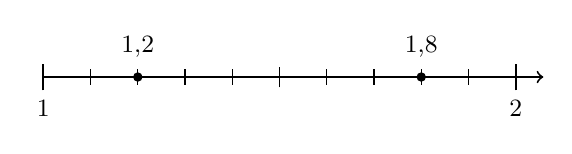
\begin{tikzpicture}[font=\small]\draw[->,line width=0.7pt] (0,0) -- (6.35,0);\draw[line width=0.7pt] (0.000,-0.17) -- (0.000,0.17);\node[below] at (0.000,-0.17) {$1$};\draw[line width=0.4pt] (0.600,-0.1) -- (0.600,0.1);\draw[line width=0.4pt] (1.200,-0.1) -- (1.200,0.1);\draw[line width=0.4pt] (1.800,-0.1) -- (1.800,0.1);\draw[line width=0.4pt] (2.400,-0.1) -- (2.400,0.1);\draw[line width=0.4pt] (3.000,-0.13) -- (3.000,0.13);\draw[line width=0.4pt] (3.600,-0.1) -- (3.600,0.1);\draw[line width=0.4pt] (4.200,-0.1) -- (4.200,0.1);\draw[line width=0.4pt] (4.800,-0.1) -- (4.800,0.1);\draw[line width=0.4pt] (5.400,-0.1) -- (5.400,0.1);\draw[line width=0.7pt] (6.000,-0.17) -- (6.000,0.17);\node[below] at (6.000,-0.17) {$2$};\fill (1.200,0) circle (1.7pt);\node[above] at (1.200,0.12) {$1{,}2$};\fill (4.800,0) circle (1.7pt);\node[above] at (4.800,0.12) {$1{,}8$};\end{tikzpicture}}{}{}
\medskip
\aufg{\hangindent7mm\hangafter1\nr{4.}Welche Zahl liegt genau in der Mitte? Hier liegt ein Einer dazwischen.\par\vspace{3pt} a)~$2{,}9$ und $3{,}2$ \qquad b)~$5{,}7$ und $6{,}4$}{}{}
\medskip
\aufg{\hangindent7mm\hangafter1\nr{5.}An einem Wanderweg steht eine Hütte bei km $3{,}4$ und eine Brücke bei km $4{,}1$. Genau in der Mitte dazwischen soll eine Bank stehen. Ein Rastplatz liegt bei km $3{,}8$. Liegt der Rastplatz zwischen Hütte und Bank oder zwischen Bank und Brücke?}{}{{\scriptsize\color{mbgrau}Ziel\hspace{2mm}}}
\medskip
\par\vspace{3mm}\setlength{\kr}{\dimexpr\pagegoal-\pagetotal-10mm\relax}%
\ifdim\kr>12mm\karomerk{k}{C}\noindent{\scriptsize\color{mbgrau}Platz zum Rechnen}\par\nointerlineskip\vspace{1mm}\noindent
\begin{tikzpicture}\clip (0,0) rectangle ({\linewidth-0.5mm},\kr);\draw[black!16,line width=0.3pt,step=5mm] (0,0) grid (\linewidth,\kr);\end{tikzpicture}\fi\par
\clearpage\label{s:D}\noindent\colorbox{black!12}{\makebox[10mm]{\Large\bfseries\strut D}}\hspace{3mm}{\Large\bfseries Bruch, Prozent, Quadrat: erst umwandeln}\par\smallskip
\noindent Bring alle Zahlen in dieselbe Form, am besten in Dezimalzahlen. Dann vergleichst du wie in A.\par\medskip
\noindent\textbf{Formel}\par\nopagebreak\noindent\hspace*{4mm}\begin{minipage}{\dimexpr\linewidth-4mm\relax}Bruch: erweitern auf 10 oder 100 \ (Nenner 2, 5 $\to$ 10; \ 4, 20, 25, 50 $\to$ 100) \par\vspace{4pt} Prozent: $p\,\% = \dfrac{p}{100}$ \qquad Quadrat: $0{,}a^2 = 0{,}a \cdot 0{,}a$\end{minipage}\par\medskip
\noindent\textbf{Beispiel}\quad Welcher Wert ist der kleinste: $\dfrac{3}{20}$; \ $0{,}3^2$; \ $5\,\%$; \ $0{,}3$?\par\smallskip
\noindent\par\noindent\hangindent6mm\hangafter1\makebox[6mm][l]{\textbf{1}}Bruch: Erweitere auf 100: $\dfrac{3}{20} = \dfrac{15}{100} = 0{,}15$.\par\smallskip\par\noindent\hangindent6mm\hangafter1\makebox[6mm][l]{\textbf{2}}Quadrat: $0{,}3^2 = 0{,}3 \cdot 0{,}3$. Rechne $3 \cdot 3 = 9$. Beide Zahlen haben zusammen 2 Stellen nach dem Komma: $0{,}09$.\par\smallskip\par\noindent\hangindent6mm\hangafter1\makebox[6mm][l]{\textbf{3}}Prozent heißt Hundertstel: $5\,\% = \dfrac{5}{100} = 0{,}05$.\par\smallskip\par\noindent\hangindent6mm\hangafter1\makebox[6mm][l]{\textbf{4}}Vergleiche wie in A: $0{,}15$; \ $0{,}09$; \ $0{,}05$; \ $0{,}30$. Am kleinsten: $0{,}05$, also $5\,\%$.\par\smallskip\par\medskip
\noindent\textbf{Aufgaben}\hspace{1em}{\small\color{mbgrau}\karohinweis{D}{Rechne unten im Karo.}{Rechne auf einem extra Blatt.} Vergleiche jede Aufgabe gleich mit dem Lösungsheft.}\par\smallskip
\aufg{\hangindent7mm\hangafter1\nr{1.}Schreibe als Dezimalzahl.\par\vspace{3pt} a)~$\dfrac{3}{5}$ \qquad b)~$45\,\%$ \qquad c)~$0{,}2^2$ \qquad d)~$7\,\%$ \qquad e)~$\dfrac{3}{4}$ \qquad f)~$0{,}6^2$}{}{}
\medskip
\aufg{\hangindent7mm\hangafter1\nr{2.}Setze $<$, $=$ oder $>$ ein.\par\vspace{3pt} a)~$\dfrac{3}{4}$ \leerfeld $0{,}7$ \qquad b)~$8\,\%$ \leerfeld $0{,}8$ \qquad c)~$0{,}7^2$ \leerfeld $0{,}7$ \qquad d)~$\dfrac{3}{20}$ \leerfeld $15\,\%$}{}{}
\medskip
\aufg{\hangindent7mm\hangafter1\nr{3.}Ordne von klein nach groß: $\dfrac{2}{5}$; \ $0{,}38$; \ $39\,\%$; \ $0{,}6^2$.}{}{}
\medskip
\aufg{\hangindent7mm\hangafter1\nr{4.}Kreuze die Aussage an, die wahr ist.\par\smallskip\leftskip7mm \kreuz{$0{,}3^2 = 0{,}6$}\ \kreuz{$\dfrac{1}{4} > 0{,}3$}\par\kreuz{$6\,\% = 0{,}06$}\ \kreuz{$0{,}9 < 85\,\%$}}{}{}
\medskip
\aufg{\hangindent7mm\hangafter1\nr{5.}Drei Klassen zählen, wer mit dem Rad zur Schule kommt. In der 6a sind es $\dfrac{3}{4}$ der Kinder, in der 6b $0{,}68$ der Kinder, in der 6c $72\,\%$ der Kinder. In welcher Klasse ist der Anteil am größten?\par\smallskip\leftskip7mm \kreuz{6a}\ \kreuz{6b}\par\kreuz{6c}}{}{{\scriptsize\color{mbgrau}Ziel\hspace{2mm}}}
\medskip
\par\vspace{3mm}\setlength{\kr}{\dimexpr\pagegoal-\pagetotal-10mm\relax}%
\ifdim\kr>12mm\karomerk{k}{D}\noindent{\scriptsize\color{mbgrau}Platz zum Rechnen}\par\nointerlineskip\vspace{1mm}\noindent
\begin{tikzpicture}\clip (0,0) rectangle ({\linewidth-0.5mm},\kr);\draw[black!16,line width=0.3pt,step=5mm] (0,0) grid (\linewidth,\kr);\end{tikzpicture}\fi\par
\clearpage\label{s:T}\noindent\colorbox{black!12}{\makebox[10mm]{\Large\bfseries\strut T}}\hspace{3mm}{\Large\bfseries Probetest}\par\smallskip
\noindent Gemischt, ohne Beispiel. Etwa 20 Minuten.\par\medskip
\noindent\textbf{Aufgaben}\hspace{1em}{\small\color{mbgrau}\karohinweis{T}{Rechne unten im Karo.}{Rechne auf einem extra Blatt.} Vergleiche jede Aufgabe gleich mit dem Lösungsheft.}\par\smallskip
\aufg{\hangindent7mm\hangafter1\nr{1.}Ordne von klein nach groß: $2{,}08$; \ $2{,}8$; \ $2{,}078$; \ $2{,}18$.}{}{}
\medskip
\aufg{\hangindent7mm\hangafter1\nr{2.}Runde.\par\vspace{3pt} a)~$7{,}348$ auf Zehntel \qquad b)~$7{,}348$ auf Hundertstel \qquad c)~$9{,}97$ auf Zehntel}{}{}
\medskip
\aufg{\hangindent7mm\hangafter1\nr{3.}Welche Zahl liegt genau in der Mitte zwischen $4{,}7$ und $4{,}8$?}{}{}
\medskip
\aufg{\hangindent7mm\hangafter1\nr{4.}Setze $<$, $=$ oder $>$ ein.\par\vspace{3pt} a)~$\dfrac{7}{20}$ \leerfeld $0{,}35$ \qquad b)~$6\,\%$ \leerfeld $0{,}6$ \qquad c)~$0{,}9^2$ \leerfeld $0{,}9$}{}{}
\medskip
\aufg{\hangindent7mm\hangafter1\nr{5.}Welcher Wert ist der kleinste? Kreuze an.\par\smallskip\leftskip7mm \kreuz{$0{,}8$}\ \kreuz{$0{,}08$}\par\kreuz{$0{,}2^2$}\ \kreuz{$7\,\%$}}{}{}
\medskip
\aufg{\hangindent7mm\hangafter1\nr{6.}Für das Klassenfest gibt es drei Krüge mit Saft und Sirup. In Krug A ist $\dfrac{1}{4}$ des Getränks Sirup, in Krug B $0{,}2$ und in Krug C $22\,\%$. Lea mag es möglichst wenig süß. Welchen Krug nimmt sie? Welcher Krug ist am süßesten?}{}{{\scriptsize\color{mbgrau}Ziel\hspace{2mm}}}
\medskip
\par\vspace{3mm}\setlength{\kr}{\dimexpr\pagegoal-\pagetotal-10mm\relax}%
\ifdim\kr>12mm\karomerk{k}{T}\noindent{\scriptsize\color{mbgrau}Platz zum Rechnen}\par\nointerlineskip\vspace{1mm}\noindent
\begin{tikzpicture}\clip (0,0) rectangle ({\linewidth-0.5mm},\kr);\draw[black!16,line width=0.3pt,step=5mm] (0,0) grid (\linewidth,\kr);\end{tikzpicture}\fi\par
\end{document}
